\section*{Process Management}
\begin{description}
    \item[Process] Program loaded into mem, in execution.
  \item[Program] Passive entity stored on disk
  \item[Process states] new, ready, running, waiting, terminated
  \item[Process Control Block] Information about each P: P state, P number, PID, program counter, CPU registers, Mem.-management information (allocated mem for process), I/O status, CPU scheduling info (e.g. priority), Accounting info (e.g. CPU used)
  \item[Context Switch] When CPU switches to another P, save PCB of prev. P, load PCB of new P. (overhead)
\end{description}

\subsection*{Processes Layout}
\begin{tikzpicture}[remember picture,overlay]
    \node[xshift=76mm,yshift=5mm] at (current page.south west){%
    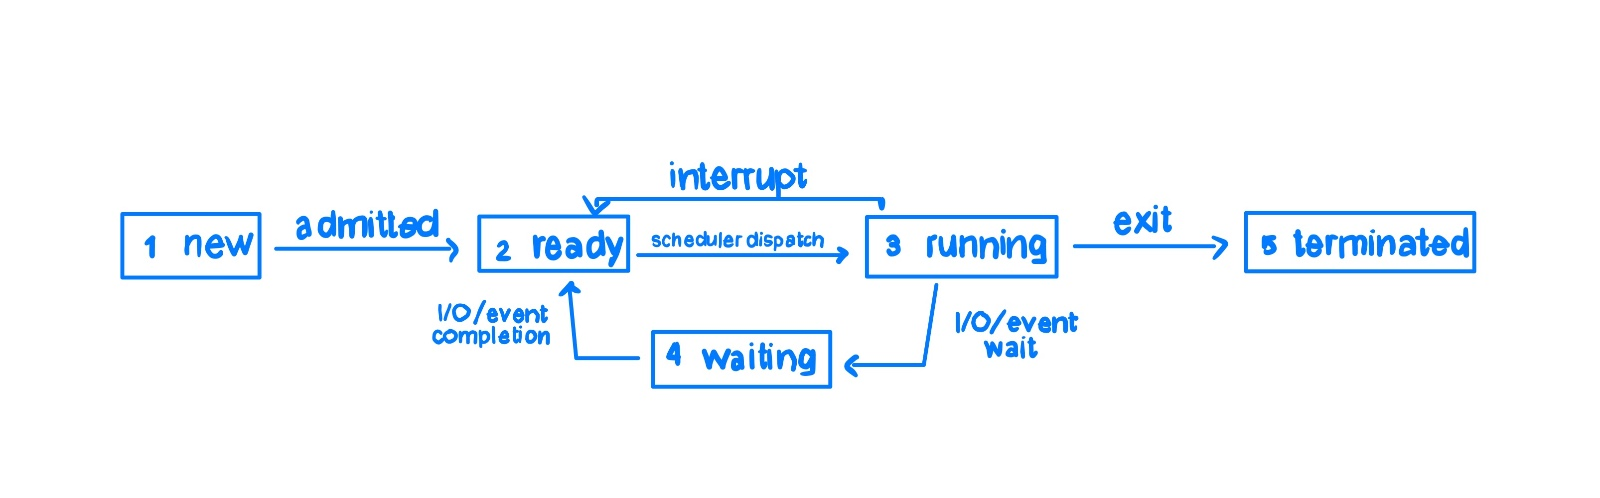
\includegraphics[width=55mm]{process_states.jpeg}};
\end{tikzpicture}
\begin{description}
  \item[Stack] temporary data: function parameters, return addresses, local variables
  \item[Heap] dynamically mem allocated during execution
  \item[data] Global variables
  \item[text] executable code
\end{description}

\subsection*{Operations on processes}
\begin{description}
  \item[Process creation]Parent P creates child (fork()) which can create own children → tree structure, every P has a unique identifier (PID). Either parent and child share all, a part or no resources.
  \item[Process termination] P's del themselves w/ exit(). Parent del child w/ abort(). Parent waits for child to end w/ wait(). child → \textbf{zombie} if child terminates before/w/o parent wait(), → \textbf{orphan} if parent terminates.
\end{description}

\subsection*{Interprocess communication}
\begin{description}
    \item[Cooperating P's](vs. Independent P's) execute concurrently, may be interrupted, share data. Need IPC
    \item[Shared Memory]Communication is under control of user P (not OS), P's share mem. space. Issue: \textbf{Producer-Consumer problem}: information to communicate stored in buffer. \textbf{unbounded:} no size limit, prod. can always produce, nice but unrealistic. \textbf{bounded:} fixed-size buffer. producer must wait if full.
  \item[Message passing] Communication controlled by OS, Messaging b/w P's w/out shared variables.\\
    \textbf{Communication Link}: \textit{Physical} (shared mem, HW bus, network). \textit{Logical}: direct/indirect, sync/async (blocking, non-blocking, rendez-vous),buffering (zero (sync r-v.)/bounded/unbounded capacity).
  \item[Direct Message passing] A link is established b/w P's. They must name each other explicitly (send(P,message), receive(Q,message)). Only one communication link. uni/bidirectional.
  \item[Indirect message passing] Messages are sent and received from mailboxes (i.e. ports). May share several communication links. uni/bidirectional.
  \item[Ordinary Pipe] Comm. b/w parent and child, cannot be accessed from outside the P that created it. Have a read end (fd[1]) and write end (fd[0]). Exists until P completion. (unidirectional)
  \item[Named Pipe, FIFO] Several P's can use pipe for communication. Exist until deleted. Appears as a file. (bidirectional: half/full duplex) %NOTE: duplex: travel one direction at the time or both at the same.
  \item[Socket] Endpoint of communication b/w machines, concatenation of IP and port. Data is sent via packets.
  \item[Remote Procedure Calls] abstract procedure (function) calls between Ps on networked systems. %NOTE: function can be invoked by P on another computer.
\end{description}
